\documentclass[french]{report}
\usepackage[utf8]{inputenc}
\usepackage[T1]{fontenc}
\usepackage{babel}
\usepackage{graphicx}
\usepackage{amsmath,amsmath,amssymb}
\usepackage{sectsty}
\usepackage{authblk}
\usepackage{algorithmic}
\usepackage[lined,commentsnumbered,boxed]{algorithm2e}
\usepackage{xspace}
\usepackage{graphicx}
\usepackage{listings}
\usepackage{xcolor}
\usepackage{mathtools}
\usepackage{mathrsfs}
\usepackage{url}
\usepackage{float}
\usepackage[top=1.5cm,bottom=1.5cm,margin=2.5cm]{geometry}

\newcommand{\HRule}{\rule{\linewidth}{0.5mm}}

\definecolor{vert}{RGB}{0,153,51}

\providecommand{\keywords}[1]{\textbf{\textit{Keywords:}} #1}
\bibliographystyle{apalike}

\usepackage{hyperref}

\graphicspath{{Images/}}
\begin{document}

\begin{titlepage}

\begin{center}

\textsc{{\LARGE Ecole nationale de la statistique \\et de l'analyse de l'information}} \\ %nom de l'école
\vspace{5mm}

\includegraphics[width=0.4\textwidth]{ensai_logo}\\[1.0 cm] %logo de l'école

\textsc{\LARGE Projet de traitement de données}\\[0.5cm]
{\Large Etudiant 1A}\\ [1cm]

% Title
\HRule \\[0.4cm]
{ \huge \bfseries Template}\\[0.4cm]

\HRule \\[1.5cm]

% Author and supervisor

\begin{flushleft} \Large
\emph{Groupe **:}\\
Prénom1 \textsc{Nom1} \\
Prénom2 \textsc{Nom2} \\
Prénom3 \textsc{Nom3} \\
\end{flushleft}

\begin{flushright} \Large
\emph{Encadrant:} \\
Prénom \textsc{Nom} \\
\emph{Responsable:} \\
Anas \textsc{KNEFATI} \\

\end{flushright}


\vfill
{\large 20** - 20**}
\end{center}
\end{titlepage} 
\begin{abstract}
*Mettez ici le résumé de ce travail (environ 10-15 lignes)* Nous présentons dans ce rapport l'étude sur les données de quelque chose \dots.
On va présenter tout d'abord ... Puis, ...
\end{abstract}
\tableofcontents

\chapter{Introduction}
Présenter le projet, vos objectifs (globalement) et les méthodes utilisées

\begin{figure}[H]
%\includegraphics[width=\textwidth]{projet_py_1er_annee}
%\caption{\label{fig:1}}
\end{figure}

\chapter{Cahier des charges}
Décrire "la maquette" de votre application : que doit-il se passer lors de l’exécution ?\newline
Effectuer des diagrammes de votre application décrivant les fonctionnalités que vous coderez (diagramme d’état/diagramme d'activité et diagramme de cas d'utilisation).

Les diagrammes suivant concerne le 'template' Python disponible sous Moodle.
\newpage
\section{Diagramme de cas d'utilisation}
\begin{figure}[!h]
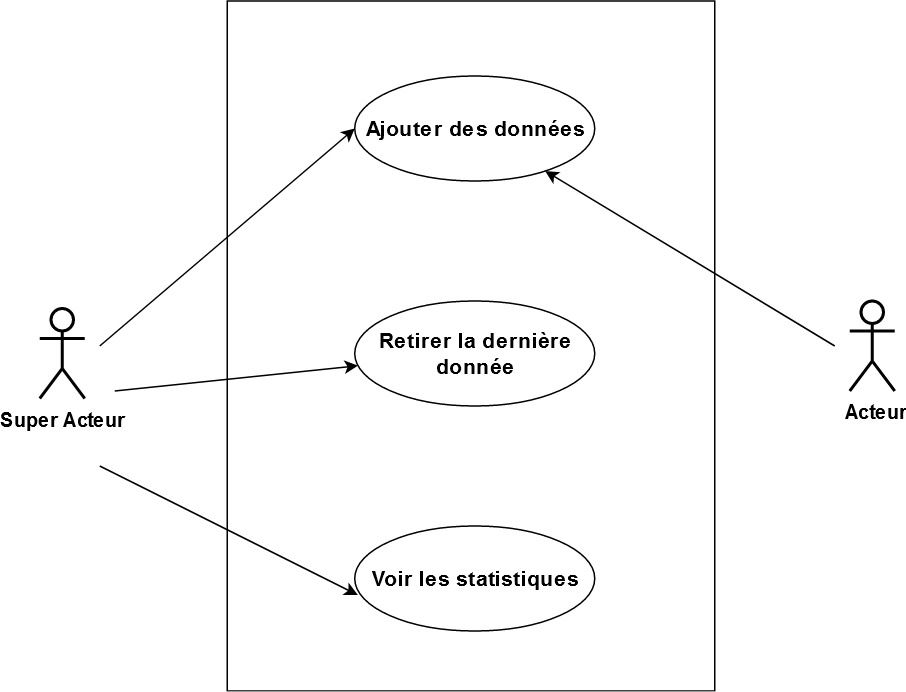
\includegraphics[width=16cm, height=16cm]{Case-Diagram.jpg}
\caption{\label{fig:1} Diagramme de cas d'utilisation}
\end{figure}
\newpage

\section{Diagramme d'activité}
\begin{figure}[!h]
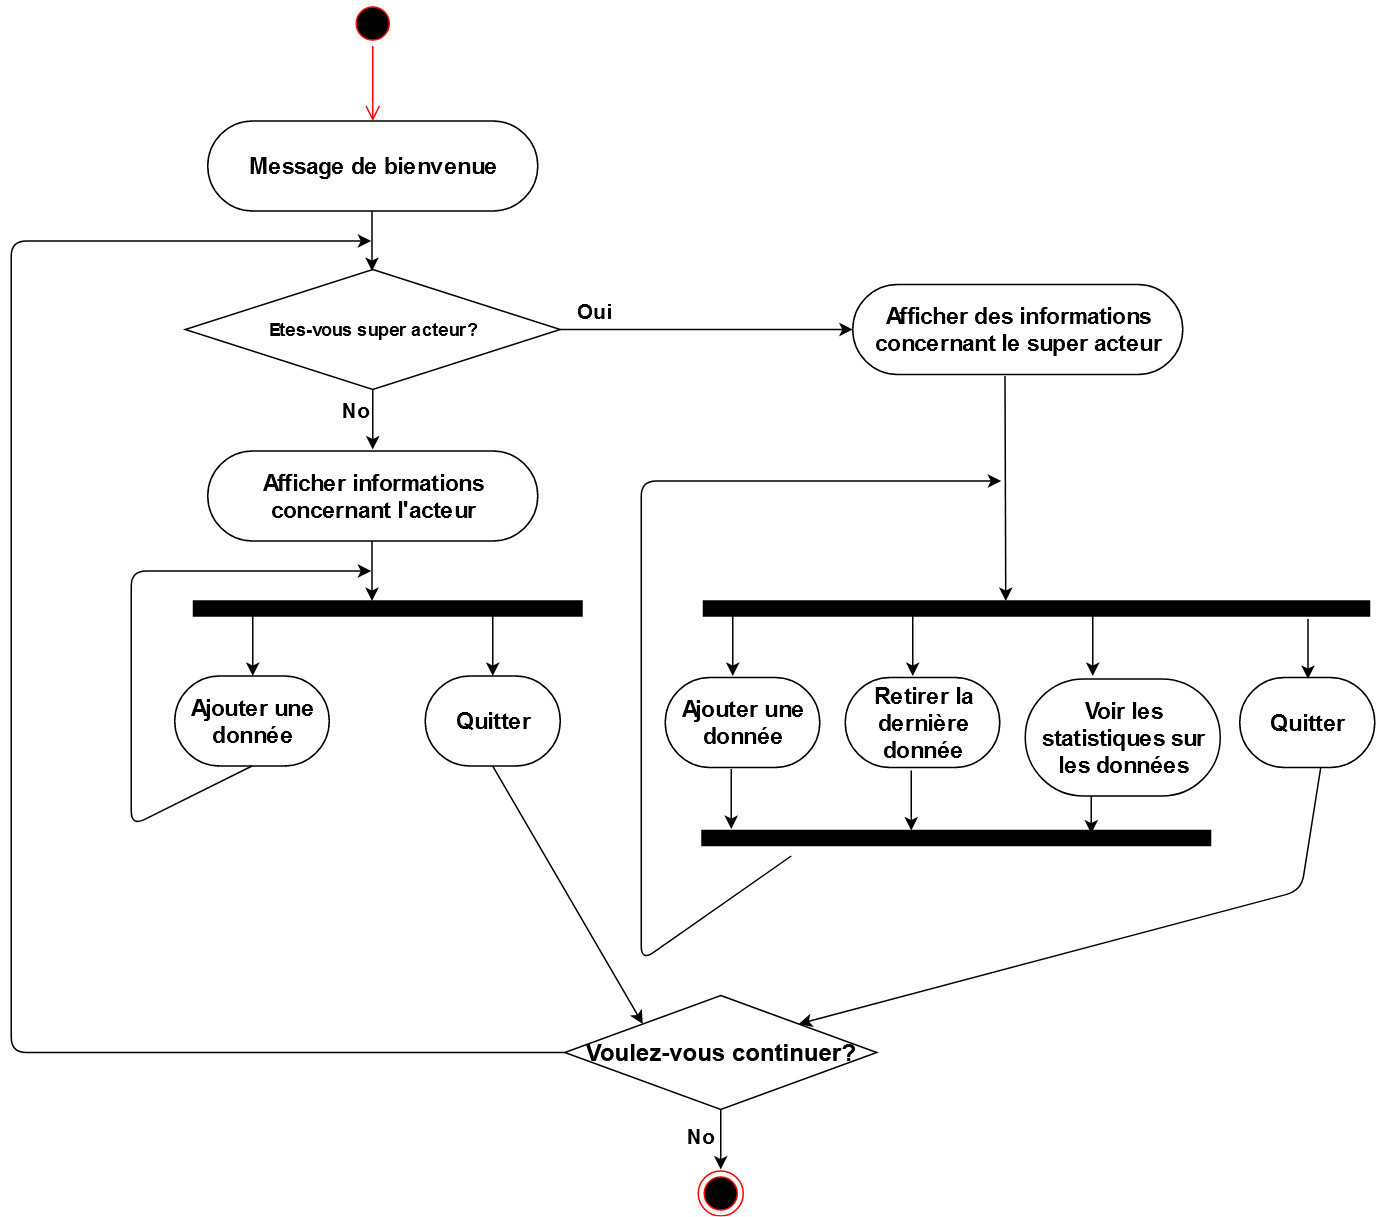
\includegraphics[width=16cm, height=18cm]{Activity_Diagram.jpg}
\caption{\label{fig:2} Diagramme d'activité}
\end{figure}
\newpage

\chapter{Architecture de l'application}
\section{Architecture de l'archive}
présenter le contenu de votre projets: Dossiers, Fichiers et le rôle de chaque dossier/fichier ainsi que le type de chaque fichier (txt, json, jpg, etc.)
Présenter les "packages", les modules, les fonctions (les signatures) ainsi que leur fonctionnalité dans chaque module.

\newpage
\section{Architecture du code}
Présenter les classes, les méthodes, les attributs de chaque classes.

\section{Diagramme de classes}
\begin{figure}[!h]
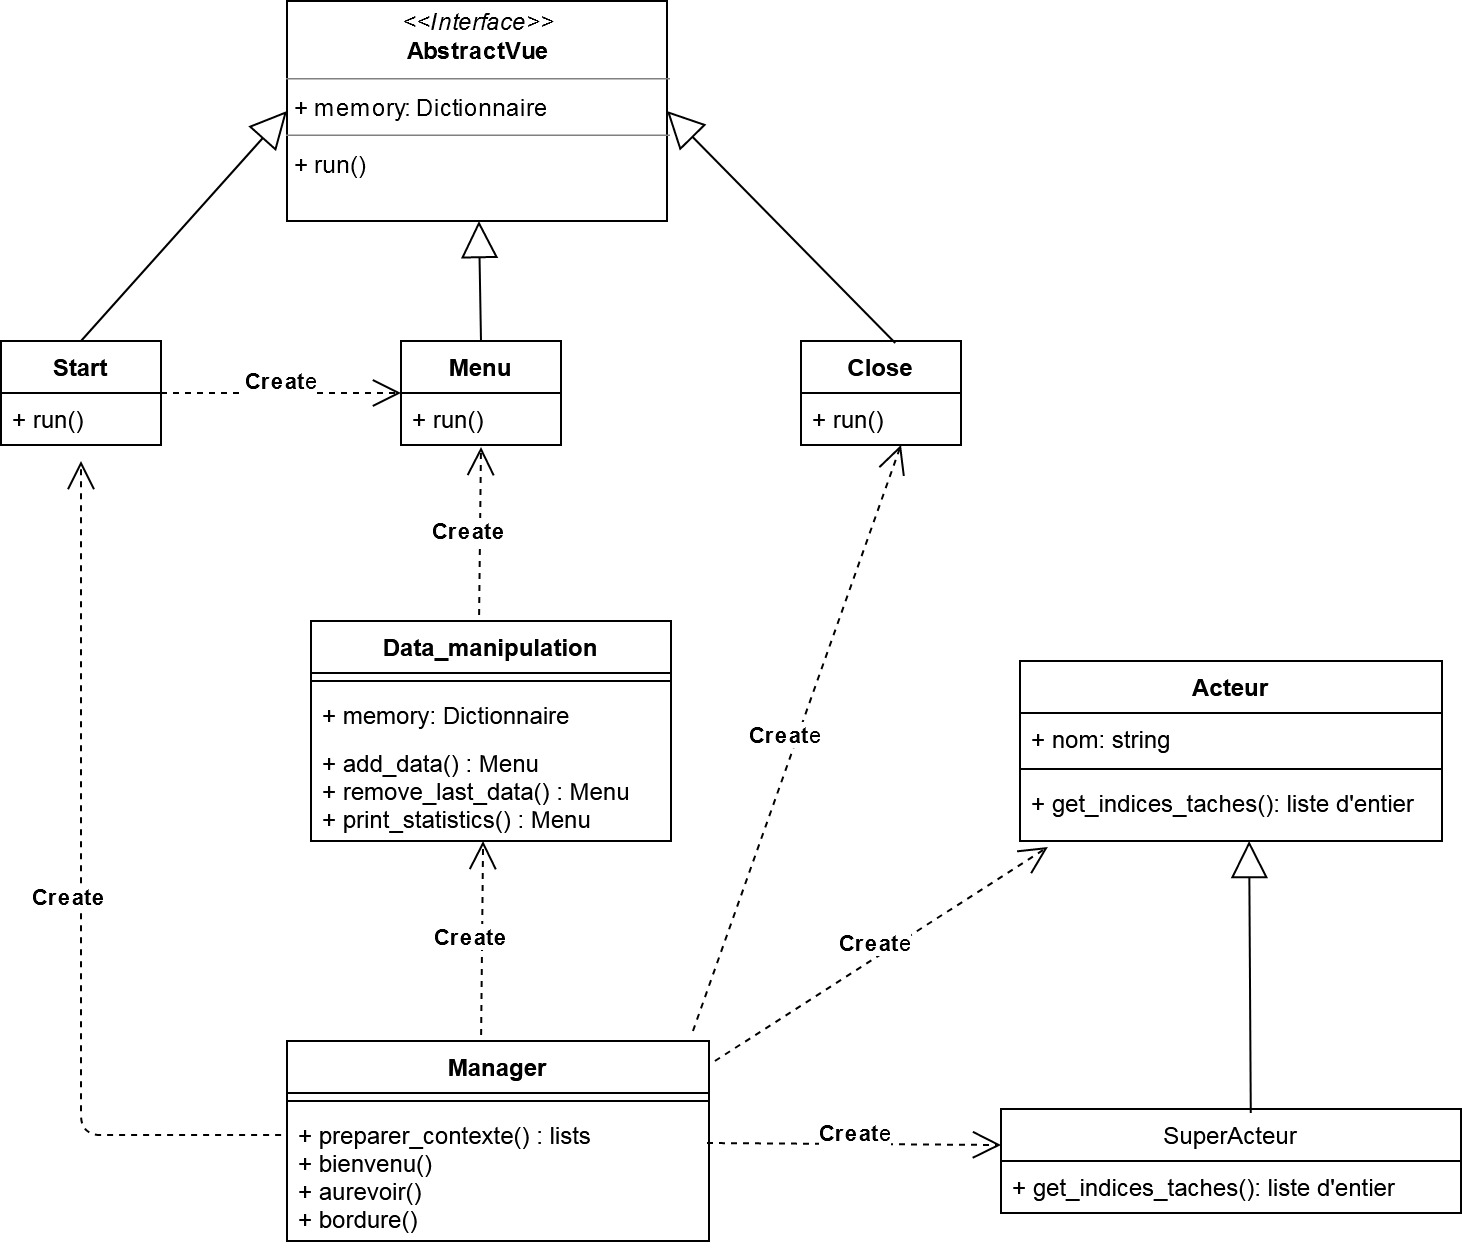
\includegraphics[width=16cm, height=18cm]{diagramme_de_classes.jpg}
\caption{\label{fig:3} Diagramme de classe}
\end{figure}


\chapter{Gestion des données}
Comment avez-vous géré les données: 
\begin{itemize}
    \item Quel type de stockage? liste , dictionnaire ou autre et pour quoi ce choix?
    \item Comment ajouter/modifier/enlever des données?
    \item Y-a-t-il un enregistrement de données sur le disque? et si oui, pourquoi et comment?
    \item etc.
\end{itemize}


\chapter{Testes}
Voir comme exemple le "template" python 
\section{Testes unitaires}
Lister les fonctionnalités que vous avez testées
\section{Teste fonctionnelle}
Expliquez le teste que vous avez fait

\chapter{Résultats}
Illustrer vos résultats ici avec les commentaires

\chapter{Répartition du travail}
Qui fait quoi, ce que vous avez appris 

\chapter{Conclusion et perspectives}
*Résumez ce que vous avez fait, présentez les résultats obtenus, donnez votre
conclusion et vos perspectives \dots *

\chapter*{Annexes}
\section{Documentation}
Présenter la documentation générée automatique à partir des commentaires dans le code.

\end{document}
